\documentclass{hbrs-ecta-report}

\usepackage{float}
\usepackage{placeins}
\usepackage{ngerman}
%\usepackage[utf8]{inputenc}
\usepackage{fontspec}
\begin{document}

\conferenceinfo{H-BRS}{2017}

\title{Neuroevolution: NeuroEvolution of Augmenting Topologies (NEAT)}
\subtitle{}

\numberofauthors{2}
\author{
\alignauthor
Tim L"ugger, Jan Urfei
}

\date{today}
\maketitle
\begin{abstract}
Aufgabe:Implementieren Sie NEAT auf den Herzfrequenz Daten. Bestimmen Sie die besten Hyperparameter. Wiederholen Sie ihr Experiment 10 mal und vergleichen Sie die Ergebnisse mit den Ergebnissen aus ESP bezogen auf die Zeit und den Error.
Plottet die durchschnittliche Elite, die Elite und den durchschnittlichen Median über alle Experimente.
Außerdem plotte die Anzahl an Knoten und Kanten über die Generationen.
\end{abstract}

\section{Herangehensweise}
\subsection{Aufbau}
 Das Erste, was wir uns überlegt haben ist, wie wir eine Topologie repräsentieren. Grundlegend haben wir zwei Listen, eine für die Knoten in einem Netz und eine für die Verbindungen (siehe Figure \ref{fig:Genomtabelle}). Das Ganze wird intern als Matrix abgespeichert, um besser damit rechnen zu können. Deswegen haben wir bei den Knoten auch den Typ in Zahlen codiert. 1 Steht für einen Input-, 2 für einen Hidden- und 3 für einen Outputknoten. Bei den Kanten steht die 1 für enabled und die 0 für disabled.
 \begin{figure}[h!]
 	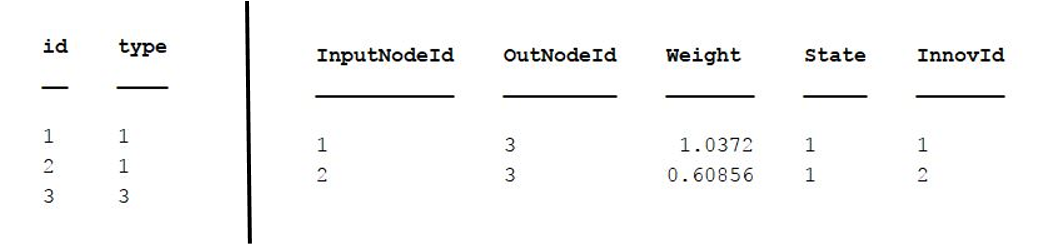
\includegraphics[width=\linewidth]{img/Genomtabelle}
 	\caption{Repräsentation eines Genoms. Links für die Knoten und rechts für die Kanten}
 	\label{fig:Genomtabelle}
 \end{figure}

Mit der Datei phenotyp.m lassen wir die Gewichtsmatrix aus den zwei oben genannten Matrizen erzeugen, um damit nachher besser rechnen zu können. Die Gewichtsmatrix, die dort zurückgegeben wird ist genauso aufgebaut wie die, die wir im ESP verwendet haben.\\
Als nächstes haben wir die Funktionen implementiert, die für die Mutation bzw. für den Crossover gebraucht werden. Die appendNode und addConnection hängen einfach nur weitere Zeilen in die in Figure \ref{fig:Genomtabelle} gezeigte Liste. Wenn Kannten hinzugefügt wird muss allerdings noch überprüft werden, ob in der gleichen Iteration schon einmal zufällig eine gleiche Innovation stattgefunden hat und wenn ja muss diese nämlich die gleiche Innovationsid bekommen. Im Zuge der Mutationen haben wir auch Funktionen geschrieben, die Kanten enablen, disablen oder switchen. Nicht alle der drei Funktionen werden im Moment verwendet, aber sie sind schon einmal da, damit spätere Erweiterungen einfacher werden.\\ 
Die Funktion mutateAdd arbeitet wie in der Vorlesung und dem Paper beschrieben. Sie erstellt einen neuen Knoten und hängt diesen zwischen zwei, wobei die alte Kante disabled wird und die eine neue Kante das Kantengewicht 1 und die andere das der alten Kante bekommt.
Die MutateAddConnection fügt eine noch nicht vorhande Kante hinzu. Dafür werden ?? zufällige Kanten erzeugt und geguckt ob eine davon noch nicht existiert. Wenn es alle schon gibt passiert nichts.
Die Funktion mutateWeights implementiert das, was in den bisherigen Algorithmen eigentlich nur gemacht wurde, und zwar die Kantengewichte anzupassen. Dazu werden zu x Prozent aller Kanten ein normalverteilter Zufallswert addiert. Wie viel Prozent verändert werden klären wir in Kapitel \ref{sec:parameter}. Der Crossover ist genau so umgesetzt, wie im Paper beschrieben.\\

Was dann noch fehlt ist eine Methode, die die Distanz zwischen zwei Netzen bestimmt, um diese nachher einer Spezies zuordnen zu können. Diese bekommt zwei Knotenlisten übergeben und muss dann erst einmal bestimmen welche die kleinere ist um diese durchgehen zu können. Die erste Liste wird also durchgegangen und bei jeder Kante wird geguckt ob sie gleich zur anderen Liste ist, disjunkt oder extra vorkommt. Je nachdem werden die Parameter E,D und W erhöht. Da es vorkommen kann, dass die zweite Liste auch Kanten hat, die in der ersten nicht vorkommen, muss ich mir die bis dorthin abgehandelten Kanten markieren und iteriere in einem zweiten Schritt noch über die nicht behandelten Kanten. Am Ende muss das Gewicht noch gemittelt werden, wie es das Paper verlangt und die Distanz mit Hilfe der Funktion $ \dfrac{c1*E}{N}+\dfrac{c2*D}{N}+c3*\bar{W}$ bestimmt werden.\\

Mit Hilfe von dieser Funktion können jetzt die Spezies eingeteilt werden. Dazu wird die erste Topologie in eine eigene Spezies gepackt. Danach wird über alle drüber iteriert und geguckt ob die Distanz unter einem gewissen Schwellwert liegt (Kapitel \ref{sec:parameter}). Wenn ja bekommt sie die gleiche Spezies wenn nicht wird eine neue eröffnet. Die Spezies werden in einem Vektor abgespeichert, indem der erste Wert für die Spezies des ersten Netzes steht. Wenn der Zielwert an Spezies nicht erreicht oder übertroffen wird, verändert sich auch der Schwellwert, für die nächste Berechnung.\\

Wie eingangs schon erwähnt wird die Berechnung des Ergebnisses eines Netzes ähnlich wie beim ESP durchgeführt, da ja auch Rekurrenz theoretisch entstehen kann. Das führt allerdings dazu, dass wenn keine direkte Kante vom Input zum Output führt das Ergebnis verzögert ist. \\

Die Methode FitnessCalulation berechnet für alle Netze die Fitness. Dafür wird pro Netz über alle Trainingszeitreihen nacheinander gegangen und der Fehler aufsummiert. Die Aktivierung von einem Netz wird nach jeder Zeitreihe aber wieder auf den Startzugang zurück gesetzt.\\

In unserem Hauptprogramm werden dann alle Funktionen im Prinzip sinnvoll hintereinander aufgerufen. Nach erstellen einer Startpopulation werden erst die Spezies bestimmt und dann die Fitness für alle berechnet. Danach sortieren wir die Population und werfen die schlechtesten raus. Für den genauen Anteil verweise ich wieder auf Kapitel \ref{sec:parameter}. Im folgenden werden die Eliten von Spezies, die mehr als 5 groß sind unverändert übernommen. Dafür suchen wir die Indizes dieser uns speichern diese. Als nächstes wird die aktuelle Größe der Population abgespeichert und die Entfernten Topologien mittels Crossover wieder aufgefüllt. Als letztes werden über die nicht Elite Topologien bis zu den neu aufgefüllten iteriert und mit einer gewissen Wahrscheinlichkeit mutiert. Der ganze Ablauf ist in Figure \ref{fig:Ablauf} nochmals grafisch dargestellt.
 \begin{figure}[t!]
	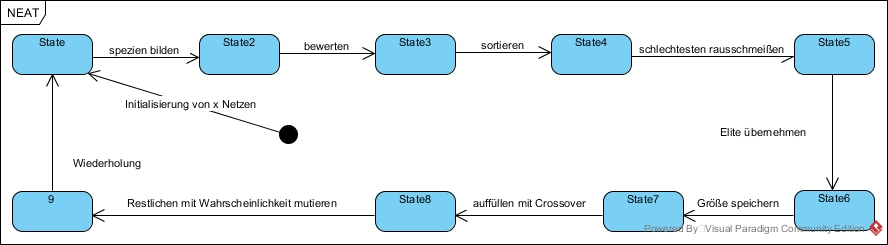
\includegraphics[width=2\linewidth]{img/Ablauf}
	\caption{Ablauf uneseres NEAT Algorithmus}
	\label{fig:Ablauf}
\end{figure}



\subsection{Hyperparameter}\label{sec:parameter}

\section{Unsere Ergebnisse}
\subsection{NeatErgebnisse}
\subsection{Verlgeich zu ESP}




\end{document}
}